\graphicspath{{./images/}}

\chapter{Konzepte}

\section{Fachliche Strukturen}

Wie in der Einführun schon erwähnt geht es bei der Applikation um das Registrieren neuer Händler für den TWINT Service. Die folgende Abbildung zeigt das Domänenmodell der Applikation. Ziel der Grafik ist es, die Struktur einfach darzustellen weshalb nicht alle Details aufgeführt sind. 

\begin{center}
	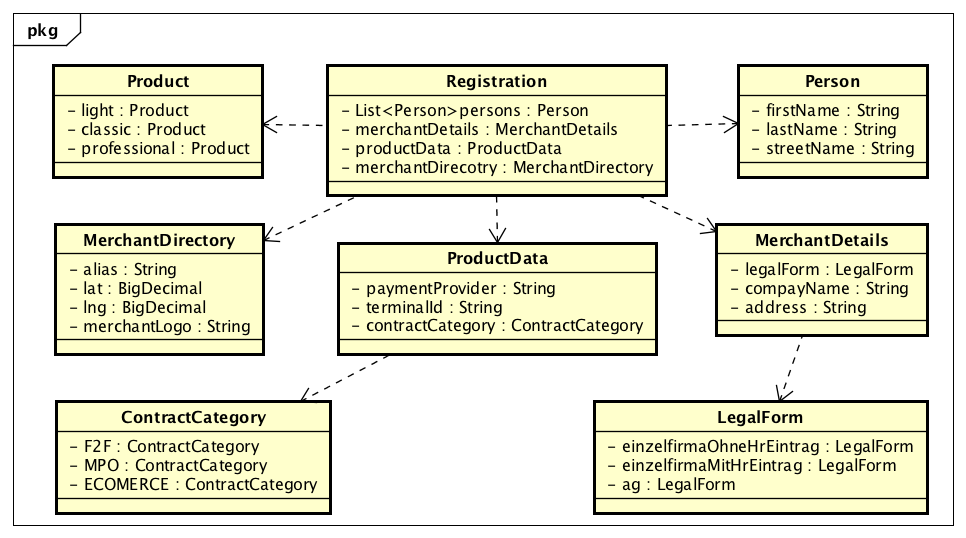
\includegraphics[scale=0.6]{DomainModel.png}
\end{center}

\section{Typische Muster und Strukturen}

\subsection{Dependency Injection}

Dieser Mechanismu stellt die korrekte zusammensetztung von Komponenten im Code sicher. Die Abhängigkeiten und Objekt Instanzierungen  müssen deshalb nicht durch den Entwickler im Code programmiert werden sondern das Framework diese Aufgabe übernimmt. Das Basis der Server Applikation bildet Spring Boot. Damit der Prozess korrekt funktioniert,
müssen entsprechende Klassen mit spezifischen Annotationen versehen werden. 
Damit Spring die Klassen beim Starten auch finden, muss entweder eine XML oder eine Java Konfiguration des Kontextes vorliegen. Darin werden die entsprechen Packages aufgelisten in welche gesucht werden soll. Eine ausführliche Erklärung der Funktionsweise findet sich unter \url{https://docs.spring.io/spring/docs/current/spring-framework-reference/html/beans.html}\newline
Im Spring Kontext wird auch oft der Name Beans verwendet wobei diese verschiedene Ausprägungen haben können. In den folgenden unter Kapiteln werden einzelne Arte genauer erklärt.\newline
Das Web Framework AngularJS verwendet ebenfalls Dependency Injection hat dafür auf Grund der Programmier Sprache JavaScript andere Modelle. Um die Abhängigkeiten aufzulösen können verschiedene Methoden verwendet werden. Eine genaue Erklärung dazu findet sich unter \url{https://docs.angularjs.org/guide/di}

\subsection{Repository}

Repositories sind eine Abstraktionschicht für die Busisses Logik welche den Zugriff auf die Datenbank abstrahiert. Sämtliche Operationen zum Speichern, Lesen und Aktualisieren, sind über Repositories zu tätigen.  Detailierte Informationen finden sich unter \url{http://docs.spring.io/spring-data/commons/docs/current/reference/html/}

\subsection{Controller}

Controller dienen als Schnittstelle zwischen einem Web Framework und einer Server Applikation. Dabei werden URL Pfad auf einem Contollermethode abbgebildet und können dadurch von einem Web Client angesprochen werden. Für moderen Applikationen wird als Transportformat JSON verwendet. Weitere Informationen unter \url{http://docs.spring.io/spring-restdocs/docs/current/reference/html5/}

\subsection{Services}

Serverseitig spricht man bei Services von Klassen welche Business Logik ausführen und somit die fachlichkeit der Applikation abbilden. Sie befinden sich in einer Schnichtenarchitektur zwischen den Controllern und den Repositories. Auf der Frontend Seite sind Services die Abstraktionschicht welche den Zugriff auf die URL auf Server Seite kapselt.

\subsection{Router}

Für die Navigation zwischen den verschiedenen Web Interface Teilen, wird in AngularJS das Konzept der Router verwendet. Sie definieren die Übergänge zwischen den einzlenen Seiten.

\section{Ausnahme- und Fehlerbehandlung}

Das Applikation hat diverse Schnittstellen zu internen und externen System. Generell wird dabei von zwischen zwei Fehler unterschieden:
\begin{itemize}
	\item Fehler welche korrigiert werden können und somit dem Benutzer nicht angezeigt werden.
	\item Fehler welche nicht korrgiert werden können und somit eine Meldung an den Nutzer zur folge haben.
\end{itemize}
Die Architektur der Applikation wurde so vorgesehen, dass der Benutzer möglichst keine Fehler des Systems bemerkt. Sämltiche Server sind redundant ausgelegt um eventuelle Netzwerkprobleme, Applikationabstürzte, Installationsprozeduren usw. abzufangen. Siehe dazu auch Kapitel \ref{deploy}. Request vom Server an die Workflow Engine werden aus diesem Grund asynchron verarbeitet.\newline
Dienste bei welchen nicht von der SIX zu Verfügung gestellt werden, sind meistens auch redunant ausgelegt, ein Fehler muss jedoch mitigiert werden. Dazu zählen die Services des Bundes, Handelsregisters und der Post. Sollte einer der Dienste bei der Registrierung nicht vorhanden sein, soll dem Benutzer eine entsprechende Meldung angezeigt werden.

\section{Build}

Jenkins, OC Plugin, Pipleline, Feature Branches

\section{Codegenerierung}

Die AngularJS Services welche die Anfragen an den Server schicken werden anhand von Swagger und den RestController automatisch während dem Build Prozess generiert. Sie können durch den Entwickler auch lokal erstellt werden wenn Änderungen gemacht wurden.

\section{Docker Container}
\label{container}
Container, welche vor allem im Zusammenhang mit Docker stehen, sind Software Einheiten mit eingenem Betreibsystem und können auf einen Host wie Linux gestartet werden. Dabei bekommen die Container einen eigenen Bereich auf dem Host System in welchem sie laufen. Dadurch kann Software als Komplettpakt, gegebenenfalls mit zusätzlichen Bibliotheken, ausgerollt werden ohne auf dem Host-System Änderungen machen zu müssen. \newline
Bevor ein Container gestartet werden kann, muss zuerst eine Definition in Form eines Dockerfiles vorliegen. Aus dieser Definition ensteht ein Image welches danach gestartet werden kann und dann als Container läuft. Container sind unverändlerlich und verlieren alle Daten welche darin gespeichert wurden. Für diesen Fall wurden persistente Volumen geschaffen welche an einen Container angehängt werden können.

\section{Bedienoberfläche}

Die Benutzeroberfläche wurde mittels des Single Page Application Frameworks Angularjs entwickelt um den Benutzer eine schnelle und einfach zu bedienende Oberfläche zur Verfügung zu stellen. 

\section{Feature Toggles}

Toggles erlaubt das Ein- und Ausschalten bestimmter Funkionalität einer Software. Ziel ist es, Änderungen welche an einer Anwendung gemacht wurden, erst zu einem späteren Zeitpunkt zu aktivieren. Für den Anwendungsfall von Continuous Deployment ist dies zwingen notwending da die während der Installattion verschieden Versionen der Software am laufen sind. Neue Funktionen können daher erst aktiviert werden wenn alle Teil der Applikation entsprechend aktualisiert wurden.

\section{Geschäftsregeln}

Obschon der Serverteil gewisse Fachlogik beinhalten, werden die Geschäftsregeln auf der Workflow Engine gemacht da nur diese auf die entsprechenden Systeme Zugriff hat. Die Engine basiert auf Camunda und wurde mit entsprechenden eingenen Klassen angereichert um den Prozess der Neuregistration für Händler durchzuführen. Der Prozess läuft aus Sicht des Benutzers asynchron ab. Je nach Ausgang sämtliche Prüfungen und Registierungen auf den entsprechenden System, erhält der neue Händern den Vertrag zugeschickt. Der Prozess läuft generell automatisch ab mit der einzigen Ausnahme, dass die \gls{PEP} Prüfung anschlägt. In diesem Fall muss die Riskabteilung eine Prüfung durchführen und eine Genehmigung erteilen. 

\section{Internationalisierung}

Das Web Interface ist mehrsprachig ausgelegt und die Sprache kann durch den Benutzer eingestellt werden. Rechtliche Dokumente sind ebenfalls in den entsprechenden Sprachen abgelegt.

\section{Kommunikation, Integration}

Als Kommunikationsmittel zwischen den einzelnen Teilen der Applikation kommen \gls{REST} und Messaging zum Einsatz. REST ist eine Art um Datenzwischen zwei System auszutauschen. Dabei werden die gängingen HTTP Methoden GET, PUT, POST und DELETE verwendet um entsprechende Aktion auf dem Schnittstelle des Zielsystems auszuführen. Als Übertragungs Format wirde JSON verwendet. Weitere Informationen finden sind unter \url{https://en.wikipedia.org/wiki/Representational_state_transfer}.\newline
Das Konfigurationmanagement von Spring Clound Config ,verwendet für die Benachrichtigung der Komponenten bei einer Konfigurationsänderung, das Messaging Protokoll \Gls{AMQP}. Die Queues werden dabei auf einem separaten RabbitMQ Server gehalt vorauf sich der Config Server und die Clients verbinden.

\section{Konfiguration}
\label{config}

Die Konfiguration der Applikation besteht aus zwei Teilen. Für die Orchestrierung der Anwendung ist gleichzeit auch die Deployment Plattform OpenShift zuständing welche bereits in Kapitel \ref{deploy} vorgestellt wurde. OpenShift verwendet intern Kubernetes für die Koordination der einzelen Teile. Die sogennannte Deployment Konfiguration basiert auf einer yaml Datei wechle bei erstellen des Projekt eingelesen werden kann. 
Um die Anwendung  auszurollen benötigt es neben Services und Container eine Beschreibung wie die Komponenten zusammenhängen. Folgende Konfigurationen müssen gemacht werden:\newline
\begin{itemize}
	\item Docker Image welches verwendet werden soll sowie die verfügbaren Ports und Protokoll.
	\item Persistente Volumen.
	\item Services auf welche zugegriffen werden muss. Diese werden dann mittels des internen DNS aufgelösst und eingetragen.
	\item Strategien was bei Konfigurations- und Containeränderungen gemacht werden soll.
	\item Eingestellungen für den Gesundheitszustand respektive ob ein Pod noch aktiv ist.
\end{itemize}

Ist die Konfiguration erstellt und in einer Datei gespeichert, kann die Anwendung jederzeit in einem neuen Projekt mit angepassten Paramatern ausgerollt werden.\newline
Der zweite Teil bilded Spring Cloud Config womit Konfiguratonänderungen zu Laufzeit ohne neustart der Applikation notwendig sind. Dafür verwendet die Bibiliothek einen zentralen Server welcher die Konfigurationen aus einem GIT Repository liest. Die Dateinamen sind nach dem Schema 'applicationname.properties' abgelegt und werden periodisch auf Änderungen überprüft. Die Client Applikation braucht ein Datei bootstrap.yml im Klassenpfad wo der Name der Applikation steht welche mit den Name des Propertyfiles übereinstimmen muss. Dadurch weiss Config Server welche Einstellungen an die Anwendung geschickt werden müssen. Damit Properties aktualisiert werden, muss die Klasse die Annotation '@RefreshScope' haben. Zusätzlich wird noch ein Bus mittels Queue, basierend auf RabbitMQ, verwendet um die Anwendungen zu benachrichtigen wenn eine Einstellung geändert hat.

\section{Logging, Protokollierung}

Sämtliche Protokollierungsdaten welche von der Applikation generiert werden, sind an den zentralen Splunk Server zu schicken.

\section{Management und Administrierbarkeit}

Da die Applikation auf OpenShift läuft wird sie auch über das Web interface oder den Command Line Client administiert. Die Firma verfolgt mittlerweile den DevOps Ansatz weshalb die Administratoren nicht die Applikation direkt verwalten, sondern sich mehr um die Plattform selber kümmern.  Das Management fällt somit dem Entwickler zu. 

\section{Migration}

Da aktuell als Datenbank MySQL verwendet wird, muss eine Migration nach MongoDB durchgeführt werden. Da die Daten von MEON durch den Wechsel von Paymit nach TWINT
obsolet werden und nur wenig Laufdaten gespeichert sind, können die Daten relativ einfach übernommen werden.

\section{Persistenz}
\label{persistenz}

Mongo DB
Replica Set

\begin{quote}
	Persistenz (Dauerhaftigkeit, Beständigkeit) bedeutet, Daten aus dem (flüchtigen) Hauptspeicher auf ein beständiges Medium (und wieder zurück) zu bringen.
	Einige der Daten, die ein Software-System bearbeitet, müssen dauerhaft auf einem Speichermedium gespeichert oder von solchen Medien gelesen werden:
	\begin{itemize}
		\item Flüchtige Speichermedien (Hauptspeicher oder Cache) sind technisch nicht für dauerhafte Speicherung ausgelegt. Daten gehen verloren, wenn die entsprechende Hardware ausgeschaltet oder heruntergefahren wird.
		\item Die Menge der von kommerziellen Software-Systemen bearbeiteten Daten übersteigt üblicherweise die Kapazität des Hauptspeichers.
		\item Auf Festplatten, optischen Speichermedien oder Bändern sind oftmals große Mengen von Unternehmensdaten vorhanden, die eine beträchtliche Investition darstellen.
	\end{itemize}
	Persistenz ist ein technisch bedingtes Thema und trägt nichts zur eigentlichen Fachlichkeit eines Systems bei. Dennoch müssen Sie sich als Architekt mit dem Thema auseinander setzen, denn ein erheblicher Teil aller Software-Systeme benötigt einen effizienten Zugriff auf persistent gespeicherte Daten. Hierzu gehören praktisch sämtliche kommerziellen und viele technischen Systeme. Eingebettete Systeme (embedded systems ) gehorchen jedoch oft anderen Regeln hinsichtlich ihrer Datenverwaltung.
\end{quote}

\section{Plausibilisierung und Validierung}

Auf dem Formular des Web Interfaces sollen Daten wie Händelername via des Unternehmensinfdentifikationserve des Bundes sowie die Addressen mittles der Services der Post überprüft werden. Angaben welcher der Händler machen muss, sind entsprechend gegenzeichnet und führen zu einem Fehler falls sie nicht validiert werden können. Der hochgeladene Handelsregisterauszug wird auf der Workflow Engine nochmals geprüft.

\section{Sessionbehandlung}

Die Applikation besitzt keine Sessions. Eine Anfrage/Bestellung eines Benutzers wird abgesendet und asynchron verarbeitet. Es gibt keine Möglichkeit sich in der Applikation einzulogen.

\section{Sicherheit}

Die Applikation befindet sich, wie im Kapitel \ref{deploy-dia} dargestellt, in zwei Verschiedenen Zonen. Der Teil in der öffentlichen Zone hält keine kritischen Informationen vor sondern Addressdaten der neuen Händler. Diese werden jnur kurzeitig für die Übertragung an die Workflow Engine gespeichert. Der Teil in der PCI Zone steht unter den gleichnamigen Compliance Anforderungen da im gleichen Bereich auch Systeme sind welche mit Kartendaten arbeiten. Aus diesem Grund ist eine entsprechende Firewall dazwischen. Diese Firewall kann jedoch kein Content Scanning durchführen weshalb vor der Workflow Engine eine Apache WebServer mit einem Security Modul steht. Der Config Server steht ebenfalls in der sicheren Zone um Passwörter zu schützen. Die ganze Kommunikation muss verschlüsselt erfolgen. Durch dem Umstieg auf OpenShift ist jedoch noch nicht klar wie die ganzen Zertifikate verwaltet werden resp. ob nur am Eingang ein offizielles verwendet wird oder ob die ganze Kommunikation verschlüsselt sein muss.

\section{Skalierung / Clusterung}

Wie bereits im Kapitel \ref{deploy} angesprochen, können auf der OpenShift Plattform die Anzahl Pods eines Services dynamisch angepasst werden. Dies kann über das WebInterface den OC Client oder über Autoscaling geschehen. Da die Applikation nur wenige tägliche Benutzer hat, wird die Skalierung manuell durchgeführt.

\section{Transaktionsbehandlung}

Im Vergleich zu klassischen \Gls{RDBMS} welche sich an die \Gls{ACID} Prizipien halten, hat MongoDB andere Mechanismen wie Transaktionen gehandhabt werden.

